\documentclass{article}
\usepackage{mainPoly}

\title{Vecteurs et translations du plan}
\date{}
\author{Seconde 9}

\begin{document}
\maketitle
\section{Définition}
\begin{tcolorbox}
\begin{definition}
Soient $A$ et $B$ deux points du plan. La \textbf{translation transformant $A$ en $B$} est une transformation géométrique qui à chaque point $C$ associe un point $D$ tel que $ABDC$ est un parallélogramme (éventuellement applati).     
\end{definition}
\end{tcolorbox}
\begin{example}

\begin{minipage}{0.45\textwidth}
\begin{center}
\begin{tikzpicture}
\draw (0,0) node[left] {$A$} -- (3,1) node[right] {$B$} -- (4,3) node[right] {$D$} -- (1,2) node[left] {$C$} -- cycle;

\draw (1,-1) node {$\bullet$} node[below left] {$E$};
\end{tikzpicture}
\end{center}    
\end{minipage}
\hfill
\begin{minipage}{0.45\textwidth}
La translation correspond à l'idée de \og glissement \fg sans rotation. La translation transformant $A$ en $B$ envoie n'importe quel point $C$ dans la même direction, le même sens et la même longueur que si l'on partait de $A$ pour arriver en $B$.

Tracer l'image de $E$ par la translation transformant $A$ en $B$.
\end{minipage}
\end{example}
\begin{remark}
Une translation dépend donc uniquement d'une \emph{direction} (car $(AB)$ et $(DC)$ sont parallèles), d'un \emph{sens} (car on s'intéresse à $ABDC$ et non pas $ABCD$) et d'une \emph{longueur} (car les longueurs $AB$ et $DC$ sont les mêmes). 

Ces trois caractéristiques sont regroupées derrière la notion de vecteur. 
\end{remark}
\begin{tcolorbox}
\begin{definition}
Un \textbf{vecteur} est un objet géométrique caractérisé par trois informations:
\begin{itemize}
\item Une direction
\item Un sens
\item Une longueur (que l'on appelle \textbf{norme})
\end{itemize}
\end{definition}
\end{tcolorbox}
\begin{definition}
Soient deux points $A$ et $B$. Le vecteur caractérisant la translation transformant $A$ en $B$ est noté $\vect{AB}$.
\end{definition}
\begin{remark}
\hfill
\begin{itemize}
\item La translation transformant $A$ en $B$ sera plutôt appelée \textbf{translation de vecteur $\vect{AB}$}.
\item Parmi les caractéristiques définissant un vecteur, il n'y a pas la \textbf{position} du vecteur dans le plan.
\end{itemize}
\end{remark}
\begin{example}
On représente un vecteur quelconque $\vect{u}$ à l'aide d'une flèche dans le plan.
\begin{center}
\begin{tikzpicture}
\draw[->] (0,0) -- (2,1.5) node[right] {$\vect{u}$};
\end{tikzpicture}
\end{center}
\end{example}
\begin{tcolorbox}
Le vecteur nul est un cas particulier de vecteur de norme nulle. Un tel vecteur n'a \textbf{ni direction, ni sens}.
\end{tcolorbox}
\newpage
\section{Opérations sur les vecteurs}
\subsection{Égalité entre vecteurs}
\begin{tcolorbox}
\begin{definition}
Deux vecteurs sont égaux si et seulement si ils ont la même direction, le même sens et la même norme.
\end{definition}
\end{tcolorbox}
\begin{example}
Soit l'héxagone régulier $ABCDEF$ de centre $O$.
\begin{center}
\begin{tikzpicture}
\coordinate (A) at ({3*cos(0)},{3*sin(0)});
\coordinate (B) at ({3*cos(60)},{3*sin(60)});
\coordinate (C) at ({3*cos(120)},{3*sin(120)});
\coordinate (D) at ({3*cos(180)},{3*sin(180)});
\coordinate (E) at ({3*cos(240)},{3*sin(240)});\coordinate (F) at ({3*cos(300)},{3*sin(300)});
\draw (A) node[right] {$A$} 
    -- (B) node[above right] {$B$}
    -- (C) node[above left] {$C$}
    -- (D) node[left] {$D$}
    -- (E) node[below left] {$E$}
    -- (F) node[below right] {$F$}
    -- cycle;
\draw (0,0) node {$\cdot$} node[above] {$O$};
\end{tikzpicture}
\end{center}
\begin{enumerate}[label=\emph{\alph*)}]
\item Représenter le vecteur $\vect{BC}$.
\item Représenter deux autres vecteurs égaux à $\vect{BC}$.
\item Représenter \textsc{le} représentant de $\vect{DC}$ ayant pour \textbf{origine} $F$.
\item Représenter \textsc{le} représentant de $\vect{BA}$ ayant pour \textbf{extrémité} $F$.
\end{enumerate}
\end{example}
\subsection{Opposé d'un vecteur}
\begin{tcolorbox}
\begin{definition}
Soit $\vect{u}$ un vecteur. Alors l'opposé de $\vect{u}$, noté $- \vect{u}$, est le vecteur ayant la même direction que $\vect{u}$, la même norme que $\vect{u}$, mais le sens \textbf{opposé} au vecteur $\vect{u}$.  
\end{definition}
\end{tcolorbox}
\begin{proposition}
Soient $A$ et $B$ deux points du plan. Alors $- \vect{AB} = \vect{BA}$.
\end{proposition}

\newpage

\subsection{Addition de vecteurs}
\begin{tcolorbox}
\begin{definition}
Soit $\vect{u}$ et $\vect{v}$ deux vecteurs. Alors la \textbf{somme de $\vect{u}$ et de $\vect{v}$}, notée $\vect{u} + \vect{v}$, est le vecteur associé à la translation résultant de l'enchaînement de la translation de vecteur $\vect{u}$ suivie de la translation de vecteur $\vect{v}$.
\end{definition}
\end{tcolorbox}
\begin{remark}
Autrement dit, $\vect{u} + \vect{v}$ décrit le glissement obtenu si l'on parcourt le trajet donné par $\vect{u}$ puis celui parcouru par $\vect{v}$.
\end{remark}
\begin{example}
Les quadrilatères $ABEF$ et $BCDE$ sont des carrés.
\begin{center}
\begin{tikzpicture}
\coordinate (A) at (0,0);
\coordinate (B) at (2,0);
\coordinate (C) at (4,0);
\coordinate (D) at (4,2);
\coordinate (E) at (2,2);
\coordinate (F) at (0,2);

\draw (A) -- (B) -- (C) -- (D) -- (E) -- (F) -- cycle;
\draw (B) -- (E);
\draw (A) node[below left] {$A$};
\draw (B) node[below] {$B$};
\draw (C) node[below right] {$C$};
\draw (D) node[above right] {$D$};
\draw (E) node[above] {$E$};
\draw (F) node[above left] {$F$};
\end{tikzpicture}
\end{center}
Tracer sur la figure les vecteurs suivants :
\begin{enumerate}[label=\emph{\alph*)}]
\item $\vect{AB} + \vect{BE}$
\item $\vect{FE} + \vect{DC}$
\item $\vect{FA} + (- \vect{DE}) + \vect{BE}$
\end{enumerate}
\end{example}
\begin{tcolorbox}
\begin{proposition}[Relation de Chasles]
Soient $A$, $B$ et $C$ trois points quelconques du plan. Alors,
\begin{equation*}
\vect{AB} + \vect{BC} = \vect{AC}\,.
\end{equation*}
\end{proposition}
\end{tcolorbox}
\begin{proposition}
Soient $\vect{u}$, $\vect{v}$ et $\vect{w}$ trois vecteurs du plan. Alors,
\begin{itemize}
\item $(\vect{u} + \vect{v}) + \vect{w} = \vect{u} + (\vect{v} + \vect{w})$
\item $\vect{u} + \vect{v} = \vect{v} + \vect{u}$
\item $\vect{u} + (- \vect{u}) = \vect{0}$ ($\vect{0}$ est le vecteur nul)
\item $\vect{u} + \vect{0} = \vect{0} + \vect{u} = \vect{u}$
\end{itemize}
\end{proposition}

\newpage

\section{Vecteurs et configurations géométriques}

\subsection{Parallélogrammes}

\begin{tcolorbox}
\begin{definition}[Rappels]
Un quadrilatère $ABCD$ est un parallélogramme si et seulement si :
\begin{itemize}
\item Les côtés opposés sont parallèles $2$ à $2$ : $(AB) \parallel (CD)$ et $(BC) \parallel (AD)$.
\item Les côtés opposés sont de même longueur $2$ à $2$: $AB = CD$ et $BC = AD$.
\item Deux côtés opposés sont parallèles et de même longueur: ($(AB) \parallel (CD)$ et $AB = CD$) ou ($(BC) \parallel (AD)$ et $BC = AD$)
\item Les diagonales $[AC]$ et $[BD]$ se coupent en leur milieu.
\end{itemize} 
\end{definition}
\end{tcolorbox}

\begin{proposition}
Soit un quadrilatère $ABCD$. Alors $ABCD$ est un parallélogramme si et seulement si $\vect{AB} = \vect{DC}$.
\end{proposition}

\begin{tcolorbox}
\begin{remark}
Attention, il ne faut \textbf{pas} vérifier $\vect{AB} = \vect{CD}$.        
\end{remark}
\end{tcolorbox}

\begin{proposition}
Soit un parallélogramme $ABCD$. Alors,
\begin{equation*}
\vect{AB} + \vect{AD} = \vect{AC}
\end{equation*}
\end{proposition}

\begin{example}
Soit $ABCD$ un parallélogramme.
\begin{center}
\begin{tikzpicture}
\draw (0,0) node[below left] {$A$} -- (3,0) node[below right] {$B$} -- (4,2) node[above right] {$C$} -- (1,2) node[above left] {$D$} -- cycle;
\draw (0,4) node {};
\end{tikzpicture}
\end{center}
\begin{enumquestions}
\item Placer sur la figure $E$, le point symétrique de $A$ par rapport à $B$. Placer sur la figure $F$, le point symétrique de $A$ par rapport à $D$.
\item Placer le point $G$ tel que $\vect{AG} = \vect{AE} + \vect{AF}$.
\item Donner la nature du quadrilatère $AEGF$.
\end{enumquestions}
\emptybox{6cm}
\end{example}

\newpage
\subsection{Milieu d'un segment}

\begin{proposition}
Soient $A$ et $B$ deux points du plan. Alors $I$ est le milieu du segment $[AB]$ si et seulement si $\vect{AI} = \vect{IB}$.
\end{proposition}

\begin{example}
\hfill
\begin{center}
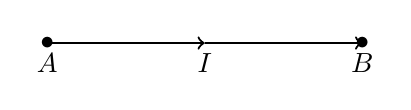
\begin{tikzpicture}
\draw[->,thick] (0,0) node[below] {$A$} node {$\bullet$} -- (2,0) node[below] {$I$};
\draw[->,thick] (2,0) -- (4,0) node[below] {$B$} node {$\bullet$};
\end{tikzpicture}
\end{center}
\end{example}

\begin{example}
Placer le milieu $I$ du segment $[AB]$ dans la figure suivante.
\begin{center}
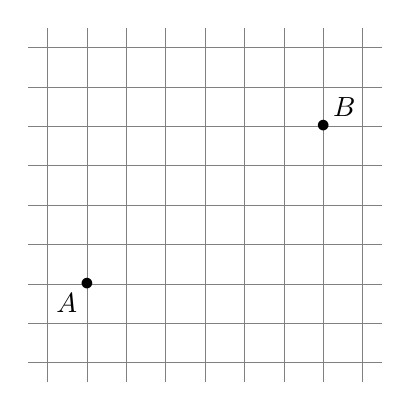
\begin{tikzpicture}
\draw[help lines] (-0.25,-0.25) grid[step=0.5] (4.25,4.25);
\draw (0.5,1) node {$\bullet$} node[below left] {$A$};
\draw (3.5,3) node {$\bullet$} node[above right] {$B$};
\end{tikzpicture}
\end{center}
\end{example}

\section{Vecteurs colinéaires}

\subsection{Multiplication d'un vecteur par un nombre réel}

\begin{tcolorbox}
\begin{definition}
Soit $\vect{u}$ un vecteur, et $k$ un nombre réel. Alors la multiplication de $\vect{u}$ par $k$ est un vecteur, noté $k\vect{u}$, vérifiant:
\begin{itemize}
\item $k\vect{u}$ est de même direction que $\vect{u}$.
\item Si $k > 0$, alors $k\vect{u}$ est de même sens que $\vect{u}$. Si $k < 0$, alors $k\vect{u}$ est de sens opposé à $\vect{u}$.
\item La norme de $k\vect{u}$ est donnée par $\abs{k}$ multiplié par la norme de $\vect{u}$.
\end{itemize}        
\end{definition}
\end{tcolorbox}
\begin{example}
Placer sur ce repére les vecteurs $2\vect{u}$ et $-3\vect{u}$.

\begin{center}
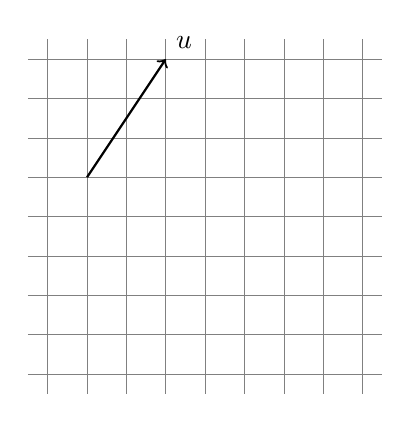
\begin{tikzpicture}
\draw[help lines] (-0.25,-0.25) grid[step=0.5] (4.25,4.25);
\draw[thick,->] (0.5,2.5) -- (1.5,4) node[above right] {$\vect{u}$};
\end{tikzpicture}
\end{center}
\end{example}

\begin{proposition}
Soient $\vect{u}$ et $\vect{v}$ deux vecteurs, et $k$ et $k'$ deux nombres réels. Alors,
\begin{itemize}
\item $k \vect{u} + k' \vect{u} = (k + k') \vect{u}$
\item $k \vect{u} + k \vect{v} = k (\vect{u} + \vect{v})$
\item $k \vect{0} = \vect{0}$
\item $0 \vect{u} = \vect{0}$
\end{itemize}
\end{proposition}

\begin{example}
Soient $A$, $B$ et $I$ trois points tels que $\vect{AI} = \dfrac{1}{2}\vect{AB}$. Montrer que $I$ est le milieu de $[AB]$.

\emptybox{2cm}
\end{example}



\newpage
\subsection{Vecteurs colinéaires et applications}
\begin{tcolorbox}
\begin{definition}
Soient $\vect{u}$ et $\vect{v}$ deux vecteurs. Ces deux vecteurs sont dits \textbf{colinéaires} si et seulement s'ils ont la même direction.
\end{definition}
\end{tcolorbox}

\begin{proposition}
Soient $\vect{u}$ et $\vect{v}$ deux vecteurs. Alors, $\vect{u}$ et $\vect{v}$ sont colinéaires si et seulement si il existe $k$ tel que $\vect{u} = k \vect{v}$. 
\end{proposition}

\begin{remark}
\hfill
\begin{itemize}
\item Pour prouver que deux vecteurs sont colinéaires, il faut donc prouver que l'un est le \textbf{multiple} de l'autre.
\item Le vecteur nul $\vect{0}$ est donc colinéaire à tous les vecteurs.
\end{itemize}
\end{remark}

\begin{proposition}
Soient $A$, $B$, $C$ et $D$ quatre points plan. Alors les droites $(AB)$ et $(CD)$ sont parallèles si et seulement si les vecteurs $\vect{AB}$ et $\vect{CD}$ sont colinéaires. 
\end{proposition}

\begin{proposition}
Soient $A$, $B$ et $C$ trois points du plan. Alors les point $A$, $B$ et $C$ sont alignés si et seulement si les vecteurs $\vect{AB}$ et $\vect{AC}$ sont colinéaires.
\end{proposition}
    
\end{document}